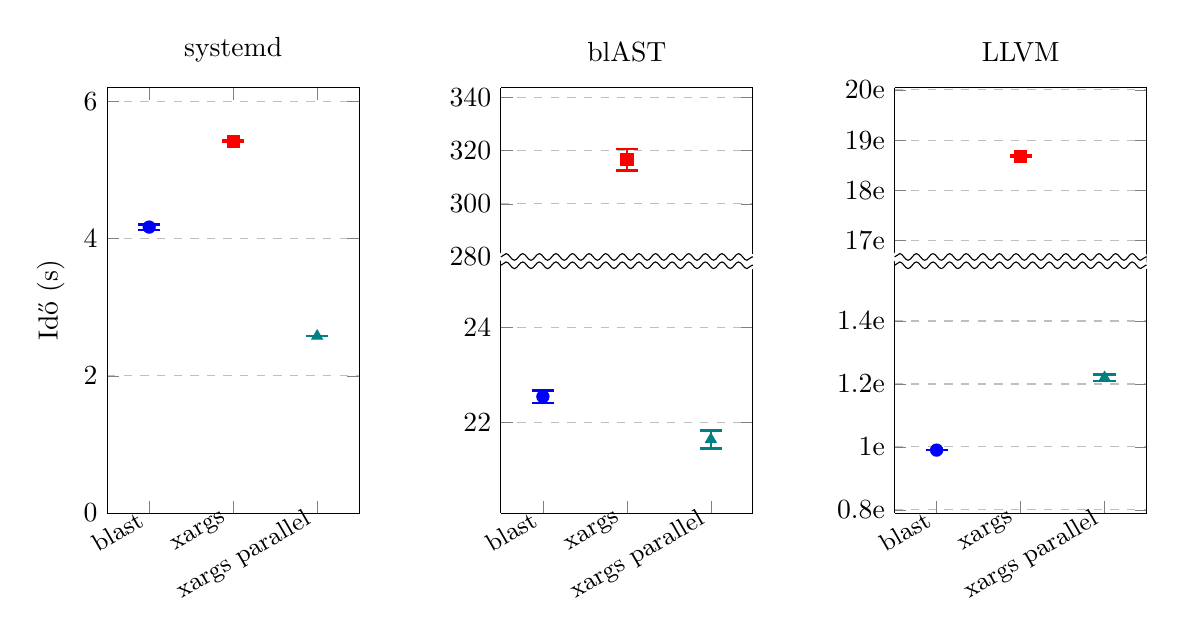
\begin{tikzpicture}
\begin{axis}[
    name=ax_sys,
    scale only axis,
    width=3.2cm,
    symbolic x coords={blast, xargs, xargs parallel},
    xtick={blast, xargs, xargs parallel},
    xmin=blast, xmax=xargs parallel,
    ymajorgrids=true,
    grid style=dashed,
    enlarge x limits=0.25,
    error bars/y dir=both, error bars/y explicit,
    error bars/error bar style={line width=0.9pt, solid},
    error bars/error mark options={rotate=90, mark size=4pt, line width=0.9pt, solid},
    height=5.4cm,
    title={systemd},
    ylabel={Idő (s)},
    ymin=0, ymax=6.2,
    xticklabel style={rotate=30, anchor=east, font=\small},
    scaled y ticks=false
]
\addplot[only marks, color=blue, mark=*, mark size=2.2pt] coordinates {(blast,4.17) +- (0.04,0.04)};
\addplot[only marks, color=red, mark=square*, mark size=2.2pt] coordinates {(xargs,5.42) +- (0.01,0.01)};
\addplot[only marks, color=teal, mark=triangle*, mark size=2.2pt] coordinates {(xargs parallel,2.58) +- (0.01,0.00)};
\end{axis}

\begin{axis}[
    name=ax_blast_top,
    at={(ax_sys.north east)},
    anchor=north west,
    xshift=1.8cm,
    scale only axis,
    width=3.2cm,
    symbolic x coords={blast, xargs, xargs parallel},
    xtick={blast, xargs, xargs parallel},
    xmin=blast, xmax=xargs parallel,
    ymajorgrids=true,
    grid style=dashed,
    enlarge x limits=0.25,
    error bars/y dir=both, error bars/y explicit,
    error bars/error bar style={line width=0.9pt, solid},
    error bars/error mark options={rotate=90, mark size=4pt, line width=0.9pt, solid},
    height=2.2cm,
    title={blAST},
    ymin=278.46, ymax=343.68,
    axis x line*=top,
    xtick=\empty,
    scaled y ticks=false
]
\addplot[only marks, color=red, mark=square*, mark size=2.2pt] coordinates {(xargs,316.61) +- (2.25,3.98)};
\end{axis}

\begin{axis}[
    name=ax_blast_bot,
    at={(ax_blast_top.south west)},
    anchor=north west,
    yshift=0pt,
    scale only axis,
    width=3.2cm,
    symbolic x coords={blast, xargs, xargs parallel},
    xtick={blast, xargs, xargs parallel},
    xmin=blast, xmax=xargs parallel,
    ymajorgrids=true,
    grid style=dashed,
    enlarge x limits=0.25,
    error bars/y dir=both, error bars/y explicit,
    error bars/error bar style={line width=0.9pt, solid},
    error bars/error mark options={rotate=90, mark size=4pt, line width=0.9pt, solid},
    height=3.2cm,
    ymin=20.10, ymax=25.40,
    axis x line*=bottom,
    xticklabel style={rotate=30, anchor=east, font=\small},
    scaled y ticks=false
]
\addplot[only marks, color=blue, mark=*, mark size=2.2pt] coordinates {(blast,22.55) +- (0.04,0.13)};
\addplot[only marks, color=teal, mark=triangle*, mark size=2.2pt] coordinates {(xargs parallel,21.65) +- (0.10,0.19)};
\end{axis}

\begin{axis}[
    name=ax_llvm_top,
    at={(ax_blast_top.north east)},
    anchor=north west,
    xshift=1.8cm,
    scale only axis,
    width=3.2cm,
    symbolic x coords={blast, xargs, xargs parallel},
    xtick={blast, xargs, xargs parallel},
    xmin=blast, xmax=xargs parallel,
    ymajorgrids=true,
    grid style=dashed,
    enlarge x limits=0.25,
    error bars/y dir=both, error bars/y explicit,
    error bars/error bar style={line width=0.9pt, solid},
    error bars/error mark options={rotate=90, mark size=4pt, line width=0.9pt, solid},
    height=2.2cm,
    title={LLVM},
    ymin=16.59, ymax=20.04,
    axis x line*=top,
    xtick=\empty,
    scaled y ticks=false,
    yticklabel={\pgfmathprintnumber{\tick}e}
]
\addplot[only marks, color=red, mark=square*, mark size=2.2pt] coordinates {(xargs,18.68) +- (0.00,0.01)};
\end{axis}

\begin{axis}[
    name=ax_llvm_bot,
    at={(ax_llvm_top.south west)},
    anchor=north west,
    yshift=0pt,
    scale only axis,
    width=3.2cm,
    symbolic x coords={blast, xargs, xargs parallel},
    xtick={blast, xargs, xargs parallel},
    xmin=blast, xmax=xargs parallel,
    ymajorgrids=true,
    grid style=dashed,
    enlarge x limits=0.25,
    error bars/y dir=both, error bars/y explicit,
    error bars/error bar style={line width=0.9pt, solid},
    error bars/error mark options={rotate=90, mark size=4pt, line width=0.9pt, solid},
    height=3.2cm,
    ymin=0.79, ymax=1.59,
    axis x line*=bottom,
    xticklabel style={rotate=30, anchor=east, font=\small},
    scaled y ticks=false,
    yticklabel={\pgfmathprintnumber{\tick}e}
]
\addplot[only marks, color=blue, mark=*, mark size=2.2pt] coordinates {(blast,0.99) +- (0.00,0.00)};
\addplot[only marks, color=teal, mark=triangle*, mark size=2.2pt] coordinates {(xargs parallel,1.22) +- (0.00,0.01)};
\end{axis}

    % blAST grafikon elszakított papír hatás
    \draw[decorate, decoration={snake, amplitude=1.2pt, segment length=6pt}, white, line width=5pt] (ax_blast_top.south west) -- (ax_blast_top.south east);
    \draw[decorate, decoration={snake, amplitude=1.2pt, segment length=6pt}, black, line width=0.4pt] ([yshift=1.5pt]ax_blast_top.south west) -- ([yshift=1.5pt]ax_blast_top.south east);
    \draw[decorate, decoration={snake, amplitude=1.2pt, segment length=6pt}, black, line width=0.4pt] ([yshift=-1.5pt]ax_blast_top.south west) -- ([yshift=-1.5pt]ax_blast_top.south east);

    % LLVM grafikon elszakított papír hatás
    \draw[decorate, decoration={snake, amplitude=1.2pt, segment length=6pt}, white, line width=5pt] (ax_llvm_top.south west) -- (ax_llvm_top.south east);
    \draw[decorate, decoration={snake, amplitude=1.2pt, segment length=6pt}, black, line width=0.4pt] ([yshift=1.5pt]ax_llvm_top.south west) -- ([yshift=1.5pt]ax_llvm_top.south east);
    \draw[decorate, decoration={snake, amplitude=1.2pt, segment length=6pt}, black, line width=0.4pt] ([yshift=-1.5pt]ax_llvm_top.south west) -- ([yshift=-1.5pt]ax_llvm_top.south east);
\end{tikzpicture}
